\documentclass[12pt,a4paper]{report}
\usepackage[utf8]{inputenc}
\usepackage[french]{babel}
\usepackage[T1]{fontenc}
\usepackage{amsmath}
\usepackage{amsfonts}
\usepackage{amssymb} 
\usepackage{mathtools}
\usepackage{xcolor}
\usepackage{graphicx}
\usepackage[left=2cm,right=2cm,top=2cm,bottom=2cm]{geometry}



\usepackage[backend=bibtex,style=authoryear,natbib=true]{biblatex}%Utilisez le backend bibtex avec le style de citation authoryear (qui ressemble à APA)
 
\addbibresource{mybiblio.bib}%le nom du fichier de la bibliographie

\usepackage[autostyle=true]{csquotes}%Nécessaire pour générer des citations dépendantes de la langue dans la bibliographie



\AtBeginDocument{\renewcommand{\labelitemi}{%
		\hspace{3mm}\textbullet}}%pour les numératation avec les puces pour les itemize



\begin{document}


%\frontmatter %Utilisez le style de numérotation des pages romain (i, ii, iii, iv...) pour les pages de pré-contenu

\pagestyle{plain}%Par défaut, le style de titre simple jusqu'à ce que le style de thèse soit appelé pour le contenu du corps

%table des matières
\tableofcontents 

\listoffigures 

\listoftables












\begin{center}
	\section{ Notion des mots clés du thème}
\end{center}


	\subsection{Notion de caméra}


Une caméra est un dispositif qui capture la lumière et la transforme en image. Elle le fait à travers une lentille, qui concentre la lumière sur une surface sensible à celle-çi, où une image se forme \cite{noauthor_quest-ce_nodate}. \\

Il ya deux catégories de caméras :
\begin{itemize}
	\item \textbf{Les caméras numériques}: qui capturent des images par voie électronique à l’aide d’un capteur.
	\item\textbf{les caméras à pellicule}: qui utilisent une bande de pellicule enduit de produits chimiques photosensibles. Elles sont utilisées pour la réalisation de film .\\
	La pellicule est une feuille mince formant le support souple à une couche sensible , elle définit chaque détaille d'une photo(couleurs, contrastes, exposition, grain, etc)\\
\end{itemize}

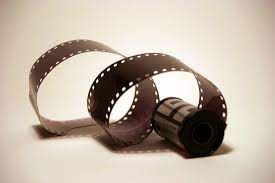
\includegraphics[scale=1]{image/pellicule.jpeg}

image d'une pellicule\\








\newpage
 
\printbibliography[heading=bibintoc]
\end{document}